\documentclass[11pt]{article}

\usepackage[utf8]{inputenc}
\usepackage[T1]{fontenc}
\usepackage[margin=2.4cm]{geometry}
\usepackage{amsmath,amssymb}
\usepackage{graphicx}
\usepackage{subcaption}
\usepackage{booktabs}
\usepackage{tikz}
\usetikzlibrary{arrows.meta,positioning}
\usepackage[hidelinks]{hyperref}
\usepackage{caption}
\captionsetup{font=small,labelfont=bf}

% Figures: keyboard frames live in ../assets, exported result frames in figures/
\graphicspath{{figures/}{../assets/}}

% Placeholder box for figures still to be exported from MATLAB.
% Replace each \figplaceholder{...} with \includegraphics[width=\textwidth]{yourfile}.
\newcommand{\figplaceholder}[1]{%
  \fbox{\begin{minipage}[c][0.32\textwidth][c]{0.96\textwidth}%
    \centering\itshape\small TODO: export from MATLAB\\[2pt]#1%
  \end{minipage}}%
}

% =====================================================================
% TITLE BLOCK  ---  FILL IN the surnames, course and date as you like.
% =====================================================================
\title{\textbf{Visual reconstruction of played notes on a piano keyboard\\
from a single top-view video}}
\author{
  Flavio De Lellis \and
  Filippo Garofalo \and
  Emanuele Turbanti \\[4pt]
  \small Image Analysis and Computer Vision -- Politecnico di Milano % TODO course/professor
}
\date{\today} % TODO set the delivery date

\begin{document}
\maketitle

\begin{abstract}
\noindent
We present a pipeline that takes an ordinary RGB video of two hands playing a
piano, filmed roughly from above, and marks on every frame which keys are being
pressed. The system uses only classical image processing and projective
geometry, with no learning involved and a single short manual calibration. Our
contribution over similar course projects is twofold. First, the keyboard is
rectified through a homography that we estimate from scratch with a normalized
Direct Linear Transform, and the key grid is then built analytically in
millimetres so that both white \emph{and} black keys are modelled. Second, the
press decision combines a spatial cue (a finger lies on the key) with a temporal
cue (the key surface actually changed), where the temporal stage uses a signed
frame difference that treats white and black keys with opposite polarity. A key
is reported as pressed only when both cues agree. We tested the method on five
videos with very different lighting, backgrounds and hand styles.
\end{abstract}

\section{Introduction}
The goal of this project is simple to state and surprisingly hard to do well:
given a video of someone playing the piano, recover which notes are sounding at
each instant, using nothing but the picture. We deliberately stay with a
single, fixed, roughly top-down camera, because that is the cheapest setup a
student or a hobbyist already owns. The output is the original video with the
pressed keys painted on top, keeping the link between each pressed key and the
finger responsible for it visible.

The motivation comes mostly from Music Information Retrieval, where automatic
transcription tries to turn a performance into a symbolic score or a MIDI
file~\cite{benetos2019transcription}. Audio based transcription is the usual
route, but it has well known trouble with dense polyphony, with notes that
overlap and with instruments that are slightly out of tune. Looking at the
player's hands sidesteps part of that, because the physical contact between a
finger and a key is unambiguous in a way that mixed audio is not. The same idea
has obvious uses in tutoring: a system that can see a wrong finger or a wrong
timing could give feedback to a student practising at home, which matters for
remote teaching.

There is also a plain computer vision reason to care. Hands on a piano are about
the worst case for hand tracking. They are not posed to help the camera, they
occlude each other constantly, fingers curl down toward the keys so the
fingertips disappear, and a finger can rest on a key without playing it. A
method that copes with this is a method that copes with a lot.

\section{Method}

\subsection{Overview}
We stay deliberately on the cheap end of the hardware spectrum: a single RGB
camera, no depth sensor and no second viewpoint, and no learned component
anywhere in the chain. Adding hardware would make the problem easier (a frontal
camera or a depth sensor measures key travel directly~\cite{akbari2015pianodepth},
and a CNN could absorb much of the appearance variation), but each of those
options carries a cost, in equipment or in annotated data, that a setup meant to
run on footage anyone can shoot should not assume. Working inside that
constraint is the whole point, and Figure~\ref{fig:pipeline} shows how we do it.

The pipeline has a one-time calibration and then a per-frame loop. Calibration
recovers the geometry of the keyboard and freezes a virtual key grid. The loop
runs two parallel branches on every frame: a \emph{spatial} branch that asks
which keys have a fingertip over them, and a \emph{temporal} branch that asks
which keys have visually changed with respect to a resting reference. A key is
declared pressed only when it appears in both branches at once. Figure~\ref{fig:pipeline}
sketches the flow.

\begin{center}
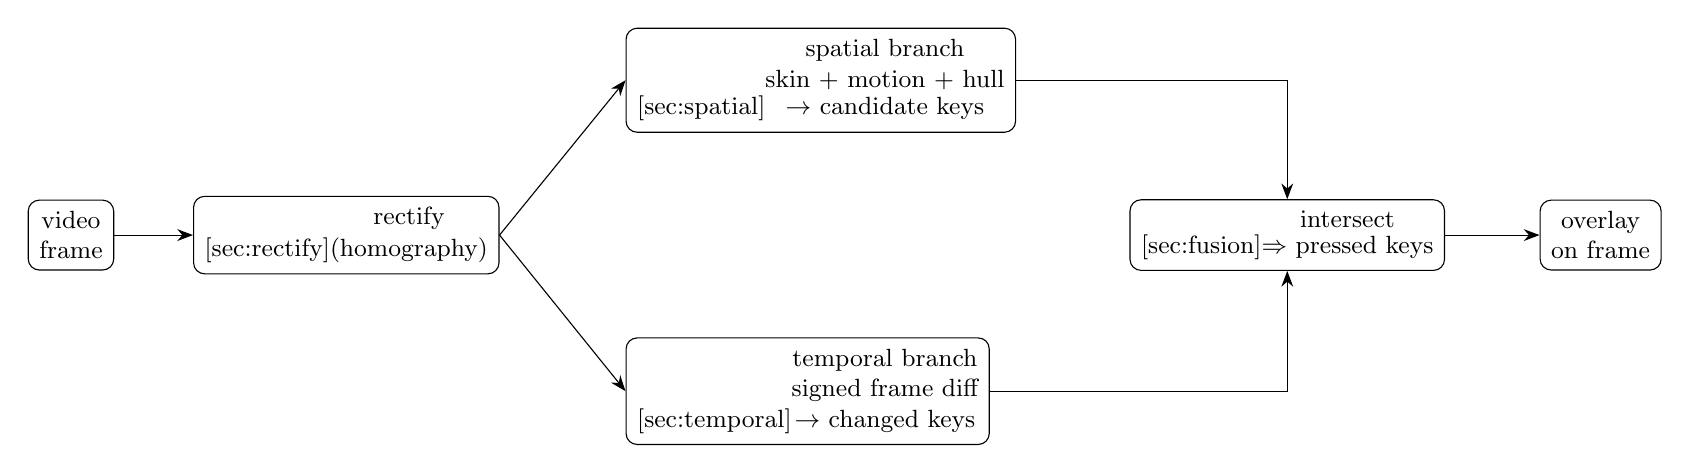
\begin{tikzpicture}[
  node distance=6mm and 9mm,
  box/.style={draw, rounded corners, align=center, font=\small, inner sep=4pt, minimum height=8mm},
  >={Stealth[length=2mm]}
]
\node[box] (frame) {video\\frame};
\node[box, right=10mm of frame] (rect) {\hyperref[sec:rectify]{\shortstack{rectify\\(homography)}}};
\node[box, above right=8mm and 16mm of rect] (spatial) {\hyperref[sec:spatial]{\shortstack{spatial branch\\skin + motion + hull\\$\rightarrow$ candidate keys}}};
\node[box, below right=8mm and 16mm of rect] (temporal) {\hyperref[sec:temporal]{\shortstack{temporal branch\\signed frame diff\\$\rightarrow$ changed keys}}};
\node[box, right=80mm of rect] (fuse) {\hyperref[sec:fusion]{\shortstack{intersect\\$\Rightarrow$ pressed keys}}};
\node[box, right=12mm of fuse] (out) {overlay\\on frame};
\draw[->] (frame) -- (rect);
\draw[->] (rect.east) -- (spatial.west);
\draw[->] (rect.east) -- (temporal.west);
\draw[->] (spatial.east) -| (fuse.north);
\draw[->] (temporal.east) -| (fuse.south);
\draw[->] (fuse) -- (out);
\end{tikzpicture}
\captionof{figure}{High level structure. Calibration (not shown) runs once and
produces the homography and the virtual key grid that both branches rely on.}
\label{fig:pipeline}
\end{center}

\subsection{Geometric calibration and rectification}
\label{sec:rectify}
Because the camera sits at a slight angle to the keyboard normal, the keys appear
as a trapezoid rather than a rectangle, and reasoning about key positions
directly in pixels is fragile. We remove this distortion with a planar
homography. The top faces of the white keys lie on a single plane $\pi$, and the
image of that plane is related to the plane itself by
\begin{equation}
  \mathbf{u} \sim \mathtt{H}\,\mathbf{x}, \qquad
  \mathbf{u}=[x,y,1]^{\top}, \quad \mathbf{x}=[X,Y,1]^{\top},
\end{equation}
where $\mathbf{x}$ is a point on the keyboard plane in millimetres and
$\mathbf{u}$ is its pixel in the frame. We do not call a library routine for
this. The operator clicks the four corners of the visible white-key region once,
those corners are ordered as top-left, top-right, bottom-right, bottom-left from
the signs of their coordinate sums and differences, and they are matched to a
metric rectangle whose width is (number of white keys) $\times 23.5$ mm and whose
height is $150$ mm.

The homography is then estimated with a Direct Linear
Transform~\cite{hartley2004multiple}. Each correspondence contributes two rows to
a $2n \times 9$ matrix $\mathtt{A}$,
\begin{equation}
\begin{aligned}
  &[-X,\,-Y,\,-1,\;0,\,0,\,0,\; xX,\,xY,\,x],\\
  &[\;0,\,0,\,0,\,-X,\,-Y,\,-1,\; yX,\,yY,\,y],
\end{aligned}
\end{equation}
and the solution is the right singular vector of $\mathtt{A}$ associated with the
smallest singular value, reshaped into the $3\times 3$ matrix $\mathtt{H}$ and
scaled so that $H_{33}=1$. We keep both $\mathtt{H}$ and its inverse, since the
two branches need opposite directions: rectifying an image needs plane to image,
while mapping a detected fingertip back onto the keyboard needs image to plane.
As a sanity check the calibration also reports the mean and maximum reprojection
error of the four corners in pixels; on our videos this stayed well under one
pixel, as expected when the input points are the same four points used to fit.

Rectification itself is done by inverse warping. We build the output grid in the
metric plane at a chosen resolution (we used $4$ pixels per millimetre), send
each output pixel through $\mathtt{H}$ into the source frame, and sample there
with bilinear interpolation. The result is a clean top-down image of the keys on
which every later step operates. The four corners double as a region of interest
mask: anything outside the clicked quadrilateral, in particular the red felt
strip above the keys that otherwise pollutes skin detection, is discarded before
segmentation. Figure~\ref{fig:rectify} shows the result on one of our frames.

\begin{figure}[t]
\centering
\begin{subfigure}{0.6\textwidth}
  \centering
  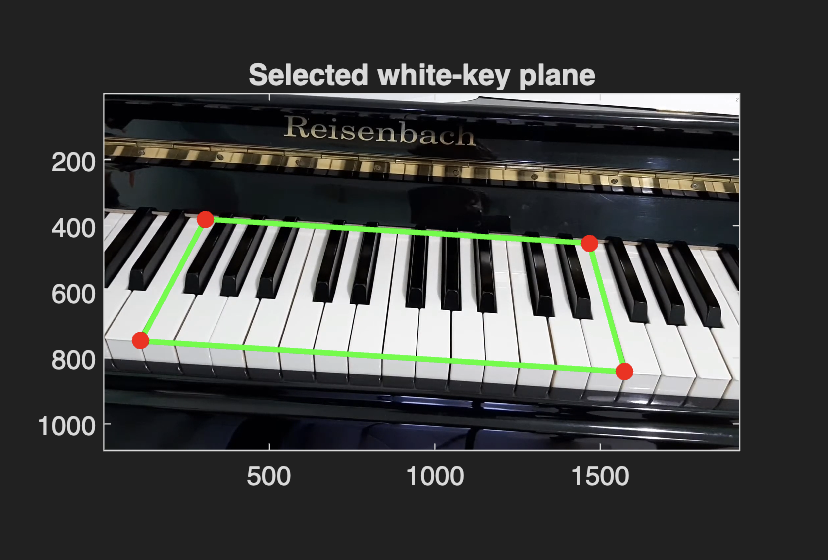
\includegraphics[width=\textwidth]{calib_corners.png}
  \caption{Source frame with the four clicked corners (red) and the resulting
  white-key quadrilateral (green), which also serves as the region of interest.}
  \label{fig:rectify-corners}
\end{subfigure}

\vspace{6pt}
\begin{subfigure}{\textwidth}
  \centering
  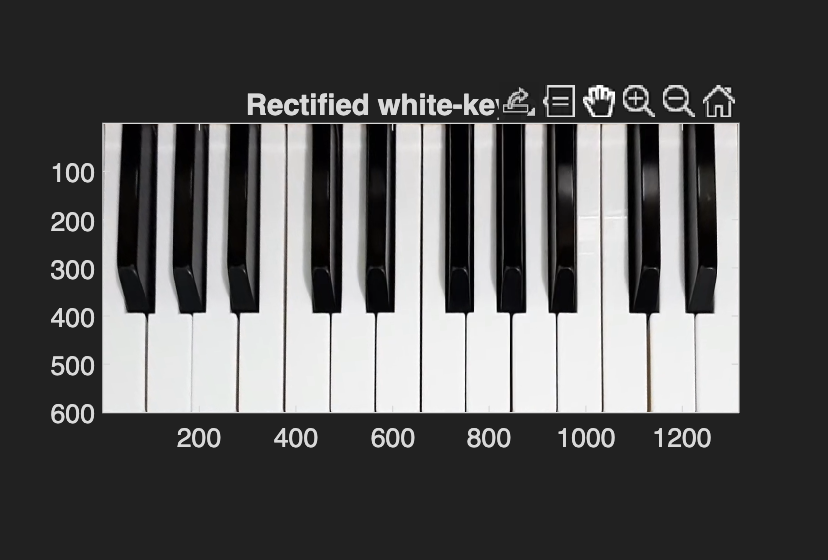
\includegraphics[width=\textwidth]{calib_rectified.png}
  \caption{The same region after inverse warping with $\mathtt{H}$: a metric,
  top-down view of the keys at $4$ pixels per millimetre.}
  \label{fig:rectify-rect}
\end{subfigure}
\caption{Calibration and rectification on a frame of one test video ($21$ white
keys, leftmost note F). The homography straightens the slanted keyboard into the
rectangular plane on which every later stage operates.}
\label{fig:rectify}
\end{figure}

\subsection{The virtual keyboard model}
Once the plane is metric we never measure key positions from the image again. We
generate them. White keys are an even partition of the calibrated width into
equal columns. Black keys are placed analytically from the standard octave
pattern $[1\,1\,0\,1\,1\,1\,0]$ (reading the white notes C,D,E,F,G,A,B, a $1$
meaning a black key sits to the right of that white). The pattern is rotated to
start on the leftmost visible note, which the user supplies, and tiled across the
visible range.

Inside each contiguous group of black keys (a pair for C\#/D\#, a triple for
F\#/G\#/A\#) we do not assume the blacks are centred on the white-white seams,
because they are not. We require instead that every white key shows the same
visible width below the black band, which gives, for a group of $N$ blacks of
width $w_b$ on white keys of width $w_w$,
\begin{equation}
  \text{gap} = w_w - \frac{N\,w_b}{N+1},\qquad
  c_i = x_{\text{left}} + i\cdot\text{gap} + \Big(i-\tfrac12\Big) w_b,
  \quad i=1,\dots,N,
\end{equation}
where $c_i$ is the centre of the $i$-th black key in the group. The constants
($w_w=23.5$ mm, $w_b=13.7$ mm, white length $150$ mm, black length $95$ mm) live
in a single file, so changing the geometry propagates everywhere with no manual
retuning. The end product is one array of keys, each carrying its polygon both
in millimetres and in rectified pixels, its bounding box and its type. This is
the shared map that the spatial and temporal branches both query. Handling black
keys at all is something the reference projects we looked at left as future work,
and the analytic placement is what made it tractable for us.
Figure~\ref{fig:vkgrid} overlays the generated grid on the rectified plane.

\begin{figure}[t]
\centering
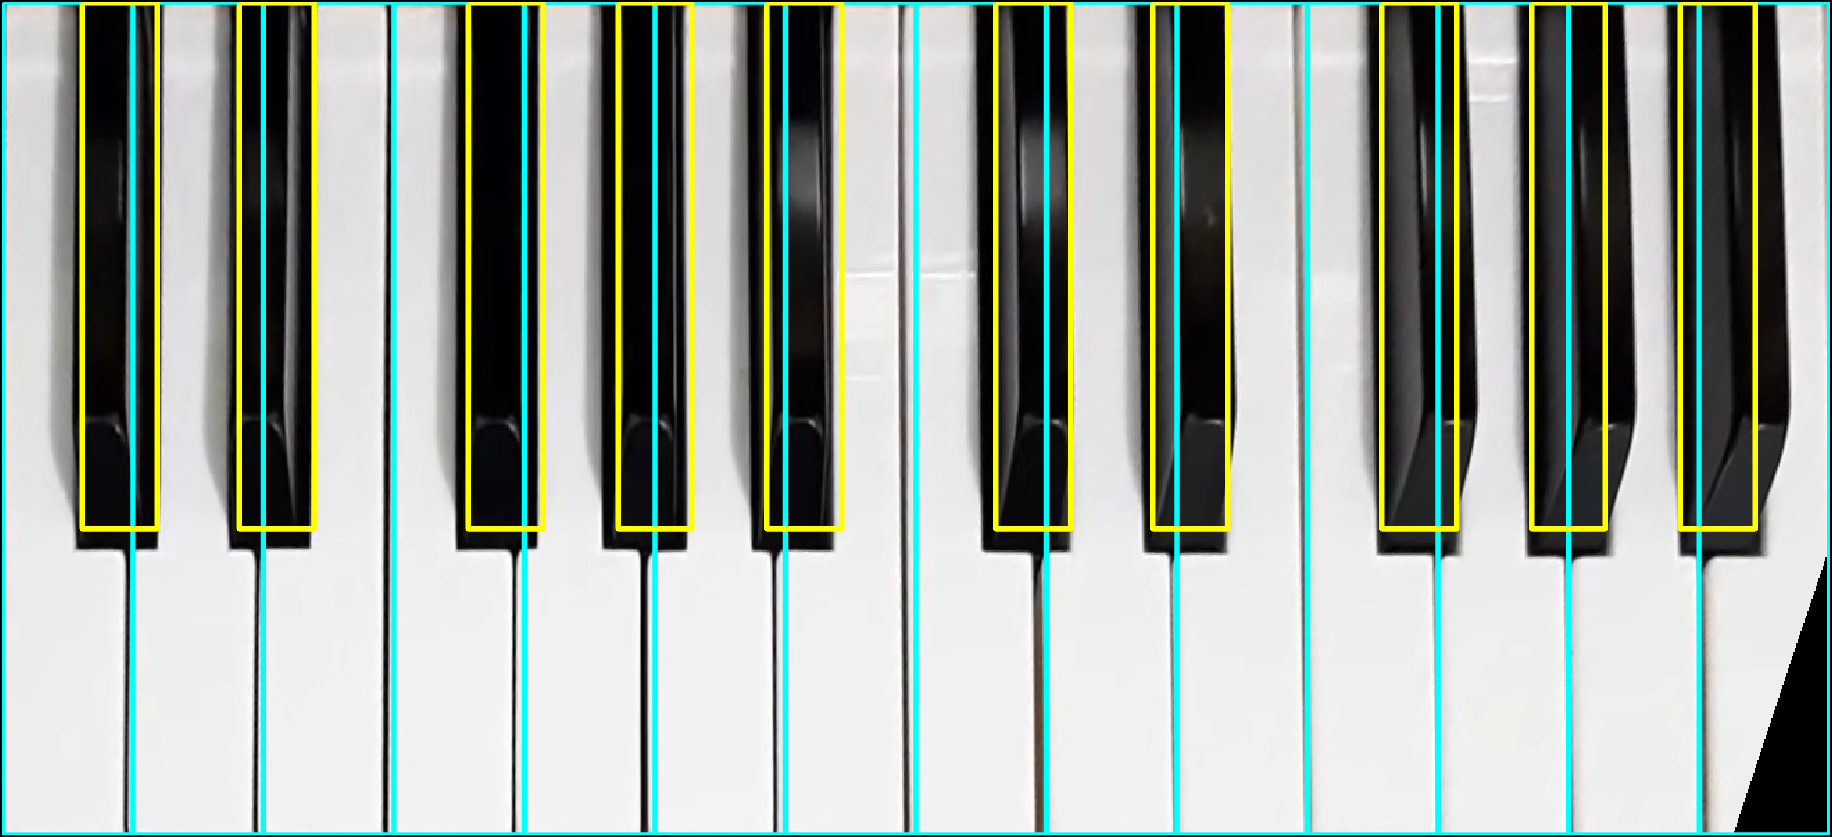
\includegraphics[width=\textwidth]{calib_grid.png}
\caption{The virtual keyboard model drawn over the rectified plane: white-key
columns in cyan and the $15$ analytically placed black keys in yellow. The grid
is computed from the two physical dimensions and the octave pattern, not measured
from the image.}
\label{fig:vkgrid}
\end{figure}

\subsection{Spatial branch: from pixels to candidate keys}
\label{sec:spatial}
The spatial branch answers a narrow question, which keys have a finger over them,
and it is allowed to over-answer, since the temporal branch will prune it.

\paragraph{Skin and motion.}
Skin is segmented in YCbCr, which separates luminance from chrominance and is a
common choice for this exact task~\cite{benabdelkader2005ycbcr}. We keep pixels
with $Y\in[100,235]$, $C_b\in[85,135]$, $C_r\in[135,180]$. On its own this also
fires on ivory keys, whose colour is close to pale skin, so we add a simple but
effective constraint: hands move and keys do not. We build a motion mask by thresholding 
the absolute grayscale difference between the current frame and the resting reference 
(using a threshold of $40$ out of $255$). Intersecting the skin mask with this motion 
mask removes the static ivory blobs that would otherwise turn into phantom fingers. 
Finally, we clean the mask with standard morphological operations, closing it with a 
$5$-pixel disk to bridge gaps, filling internal holes, and dropping any isolated 
components smaller than $50$ pixels.

\paragraph{Separating the two hands.}
We apply connected component labeling to isolate independent blobs. We keep at most 
the two largest components, provided their area $A_i$ satisfies an adaptive floor:
\begin{equation}
    A_i \geq \max\left(1000,\, 0.4 \times \max_j A_j\right)
\end{equation}
The relative term is what lets a real second hand through while still rejecting a 
distant reflection or shadow: a true second hand has an area comparable to the 
dominant component, whereas a reflection does not.

\paragraph{Fingertips by convex hull.}
Because a hand is a highly non-convex shape with deep valleys between the fingers, 
its raw contour is complex to track. To find the fingertips, we instead compute the 
convex hull of each hand blob. Intuitively, the convex hull is the shape a rubber 
band would take if stretched around the entire hand; the points where the band is 
forced to bend sharply are the protruding fingertips. 

We compute this using a custom implementation of the Graham scan~\cite{graham1972convexhull}. 
The algorithm begins by finding an anchor point guaranteed to be on the outer boundary: 
the pixel with the lowest $y$-coordinate (the base of the hand in the image), breaking 
ties with the smallest $x$-coordinate to yield $p_0 = (x_0, y_0)$. We then imagine a ray 
sweeping counter-clockwise from this anchor and sort every other pixel $p_i = (x_i, y_i)$ 
by its polar angle $\theta_i = \text{atan2}(y_i - y_0, x_i - x_0)$.

With the points sorted, we build the hull perimeter by pushing points onto a stack. 
To ensure the boundary always remains convex, we test the last three points: $p_1$ 
(second to top of stack), $p_2$ (top of stack), and $p_3$ (the new candidate). 
We calculate the 2D cross product of the vectors forming this turn:
\begin{equation}
    CP = (x_2 - x_1)(y_3 - y_1) - (y_2 - y_1)(x_3 - x_1)
\end{equation}
If $CP > 0$, the path makes a valid left turn, and $p_3$ is pushed onto the stack. 
If $CP \le 0$, the path makes a right turn, meaning $p_2$ forms a concavity (such as 
the webbing between two fingers). We pop $p_2$ off the stack, pulling the boundary 
tight over the gap, and repeat the test.

The resulting hull gives us the outer boundary points of the hand, but this includes 
the sides of the palm and the wrist. We isolate the functional fingertips using three 
spatial heuristics. First, we calculate the robust median $y$-coordinate of the hand 
blob and instantly discard any hull vertex falling below this horizontal bisector. 
Second, because a single rounded fingertip might trigger a cluster of adjacent vertices, 
we merge any candidates closer than $35$ pixels. Crucially, during this merge, we 
retain the coordinates of the candidate with the minimum $y$-value, ensuring the logged 
point correctly represents the absolute physical apex of the finger. Finally, we discard 
any vertex within $20$ pixels of the frame border, as hands cut off by the camera's 
field of view produce artificial hull corners. 

\paragraph{Mapping fingertips to keys.}
Each fingertip, detected in the original frame as homogeneous coordinates $\mathbf{u} = [x, y, 1]^\top$, 
is mapped to the rectified metric plane $\mathbf{x}_{rect}$ via the inverse homography matrix:
\begin{equation}
    \mathbf{x}_{rect} \sim \mathtt{H}^{-1} \mathbf{u}
\end{equation}
We then test black keys before white ones, because a black key physically sits on top 
of the rear portion of the whites. The test is not exact, though, and the reason is 
parallax. The homography is calibrated on the plane of the white keys. However, black 
keys and knuckles lie at an elevation above that plane, causing their projection to 
shift artificially forward in the image. We compensate for this with vertical 
tolerances tuned on the videos: $80$ pixels of slack when testing black-key boxes 
and $60$ pixels when testing white-key polygons. A fingertip matches the first black 
box that contains it (within tolerance); otherwise, it is shifted back and tested 
against the white polygons.

\paragraph{Candidate expansion across a chord.}
A finger rarely sits dead centre on a key, and a hand spanning a chord often
triggers only some of the keys it actually covers. When two or more candidates
are present, we sort them horizontally. We split them into separate groups wherever 
the spatial gap between consecutive candidates exceeds three white-key widths, 
which effectively detects the empty space between the left and right hands. 
Each group is then filled in to span its full horizontal extent. In this way, a hand 
resting across several keys reports all of them as spatial candidates, while the 
empty gap between the two hands is logically preserved.

\subsection{Temporal branch: did the surface actually change?}
\label{sec:temporal}
The spatial branch (Section~\ref{sec:spatial}) cannot tell a pressed key from a
key that is merely touched or hovered over, because from a top view the two look
almost identical: in both cases a finger sits above the key. What distinguishes a
real press is that the \emph{appearance} of the key surface changes with respect
to its resting state, while a hovering finger leaves the surface essentially
untouched. The temporal branch is the stage I designed and implemented to capture
exactly that change. It is implemented in \texttt{detectPressedKeys.m}, with the
per-frame orchestration (reference handling, skin-mask rectification, adaptive
analysis band and threshold profile) living in \texttt{main.m}. The remainder of
this section walks through it step by step.

\paragraph{Step 0 -- The resting reference.}
Every comparison is made against a single \emph{resting reference} frame, taken to
be the first rectified frame of the video (\texttt{ref\_rect} in
\texttt{main.m}). Working in the rectified, metric plane means the reference and
the current frame are pixel-aligned by construction: a given key occupies exactly
the same pixels in both, so a plain pixel-wise difference is meaningful and no
registration is needed. Importantly, the reference is allowed to already contain
the hands, as long as the keys themselves are at rest. This is what makes the
method usable on real footage, which essentially never starts on a perfectly empty
keyboard.

\paragraph{Step 1 -- Signed grayscale difference.}
The core of the branch, and the design decision I am most satisfied with, is that
I do \emph{not} use the absolute frame difference that is the textbook default.
Both frames are converted to grayscale and subtracted with their sign preserved,
\begin{equation}
  g(i,j) \;=\; \text{gray}\big(\text{current}\big)(i,j)
            \;-\; \text{gray}\big(\text{reference}\big)(i,j),
  \label{eq:signeddiff}
\end{equation}
so that the \emph{direction} of the brightness change is retained. The sign is
physically informative. A fingertip is darker than the ivory of a white key, so
pressing (or covering) a white key drives its surface darker, $g<0$. Conversely a
fingertip, and the skin around it, is lighter than the matte black of a sharp/flat
key, so acting on a black key tends to drive its surface lighter, $g>0$. The two
key families therefore live on opposite sides of zero, and I split the signal
accordingly into two non-negative channels:
\begin{equation}
  d_{\text{white}} = \frac{\max(0,\,-g)}{255}, \qquad
  d_{\text{black}} = \frac{\max(0,\;\,g)}{255}.
  \label{eq:twochannels}
\end{equation}
The decisive benefit is that the two key types stop interfering with each other.
The darkening produced by a pressed white key, including the darkening that bleeds
sideways onto its neighbours, only ever feeds the white channel $d_{\text{white}}$
and is invisible to the black channel, and the brightening produced near a black
key only ever feeds $d_{\text{black}}$. With an absolute difference the two would
be mixed, and the strong darkening of a white press is precisely what used to leak
into adjacent black keys and trigger them falsely.

\paragraph{Step 1b -- A pragmatic exception for the black channel.}
In practice a black press is weaker and more ambiguous than a white one, so I
treat the black channel with one deliberate refinement. The dominant cue when a
black key is acted upon is not only the small, narrow patch of skin that
\emph{brightens} the key, but also the \emph{shadow} that \emph{darkens} it: the
key drops, the finger casts a shadow, and the borders it shares with the
neighbouring white keys go dark. Using brightening alone lost many black presses
--- in fact the white channel often ``saw'' the black keys better than the black
channel did. I therefore compute the black channel from the \emph{magnitude} of
the signed difference,
\begin{equation}
  d_{\text{black}} = \frac{\lvert g \rvert}{255},
\end{equation}
combining both brightening and darkening, which tracks black presses far more
reliably. This is computed on the \emph{raw} $g$ of Equation~\eqref{eq:signeddiff},
before the skin mask of Step~2 zeroes anything, because for a black key the skin
is signal rather than noise. The cost of going back to a magnitude here is that it
reopens the cross-talk risk (the darkening of a pressed white bleeding onto the
edge of an adjacent black). I contain it on two fronts: the spatial intersection
downstream (Section~\ref{sec:fusion}) requires a fingertip over the black key
before it can be confirmed, and the black area threshold is raised (Step~4) so a
thin strip of edge bleed never covers enough of the key to fire it.

\paragraph{Step 2 -- Skin masking, asymmetrically.}
The rectified skin mask produced by the spatial branch (warped into the metric
plane with the same homography $\mathtt{H}$, then thresholded) is subtracted from
the \emph{white channel only}: I set $g(i,j)=0$ wherever skin is present before
forming $d_{\text{white}}$. The reason is that on a white key the moving hand
itself is a darkening event, and without this gate the finger sliding over nearby
white keys would register as a press on them. On the black channel I deliberately
do \emph{not} remove the skin, because there the brightening skin is part of the
useful press signal; zeroing it would throw away exactly what I want to detect.
This asymmetry --- skin is noise on white, signal on black --- is the second place
where the two channels are handled differently on purpose.

\paragraph{Step 3 -- Thresholding and de-speckling.}
Each channel is binarized against a per-type threshold, $\tau_{\text{white}}$ and
$\tau_{\text{black}}$ (defaulting to $20/255$ and $25/255$ in
\texttt{detectPressedKeys.m}, and raised to $30/255$ in the integrated pipeline to
suppress trigger-happy behaviour under our test lighting):
\begin{equation}
  B_{\text{white}} = \big[\,d_{\text{white}} > \tau_{\text{white}}\,\big],
  \qquad
  B_{\text{black}} = \big[\,d_{\text{black}} > \tau_{\text{black}}\,\big].
\end{equation}
The threshold may be either a scalar or a full $H\times W$ map of the same size as
the rectified image. The map variant lets the threshold vary along the keyboard to
absorb non-uniform lighting and shadows --- raised where shadows would create false
positives, lowered where genuine presses are faint --- at no per-frame cost, since
the element-wise comparison is no more expensive than the scalar one. In
\texttt{main.m} the map is built once by interpolating (\texttt{pchip}) a small set
of multiplicative gains across the keyboard width, so the spatial threshold profile
is paid for only at setup time. Each binary mask is then cleaned with a
morphological opening using a small disk ($2$\,px radius) to remove isolated
speckle that would otherwise inflate the per-key counts.

\paragraph{Step 4 -- Adaptive vertical analysis band.}
I do not analyse the whole height of each key. The lower part of the rectified
image is dominated by the moving forearm and the front of the hand, which produce
large but irrelevant differences. The original design used a fixed top third of
the keyboard; I replaced it with an \emph{adaptive} upper band. From the projected
fingertips (\texttt{fingertips\_rect\_px}) the orchestration in \texttt{main.m}
takes the smallest $y$ (the topmost fingertip), backs off a small safety margin
($10$\,px), and uses that as the cut, with a hard floor at $15\%$ of the keyboard
height so the band never collapses:
\begin{equation}
  \text{rows} = \max\!\Big(\,y_{\text{top finger}} - 10,\;\;
                 0.15 \times H_{\text{keyboard}}\,\Big).
\end{equation}
Crucially the cut is derived from the \emph{fingertips}, not from the warped skin
mask. The homography is calibrated on the plane of the white keys, but the hand is
physically above that plane, so warping the skin mask pulls the skin pixels
upward (small $y$) through parallax and would always place the cut at the very
top. The fingertips reflect the true visual position of the hand far better. If no
fingertip is detected the branch falls back to the fixed top-third behaviour.

\paragraph{Step 5 -- Per-key occupancy decision.}
For every key in the shared virtual map I take its bounding box, clip it
vertically to the analysis band of Step~4, and shrink it by a $2$\,px inner margin
on each side to reduce bleed from the adjacent keys. Inside that inner region I
read the corresponding binary channel ($B_{\text{black}}$ for black keys,
$B_{\text{white}}$ for white keys) and compute the fraction of ``on'' pixels,
\begin{equation}
  r_k = \frac{1}{\lvert R_k \rvert}\sum_{(i,j)\in R_k} B_{\text{type}(k)}(i,j),
\end{equation}
the per-key occupancy ratio. The key is reported as \emph{changed} when this
fraction exceeds a per-type level: $10\%$ for white keys and $20\%$ for black
keys. The black level is the higher of the two on purpose --- it is the anti
cross-talk guard mentioned in Step~1b, set so that a thin sliver of darkening bled
from a neighbouring white press cannot, on its own, reach one-fifth of the black
key's area, whereas a genuine press (skin plus shadow) easily does. The function
also returns, for debugging, the raw difference, both binary masks, and the vector
of per-key ratios, which I used to tune every threshold above by watching how
close each key sat to its trip level frame by frame.

\paragraph{Step 6 -- Shadow-aware region shift.}
A press does not darken only the key it lands on; it casts a shadow to one side. To
make each key capture \emph{its own} variation rather than the neighbour's, the
temporal regions can be translated by a configurable offset
(\texttt{GRID\_SHIFT\_X\_PX}, \texttt{GRID\_SHIFT\_Y\_PX}) before the per-key
counting, while the spatial branch keeps using the unshifted map. On our footage a
small horizontal shift toward the shadow side is enough to noticeably sharpen the
attribution of a press to the correct key.

\paragraph{An earlier weighted-difference variant.}
Before settling on the signed two-channel formulation I implemented and tested a
different temporal stage, preserved in \texttt{confirmPressedKeys.m}. There I took
the \emph{absolute} difference $D=\lvert\,\text{current}-\text{reference}\,\rvert$
inside each candidate key and reduced it to a single weighted mean,
\begin{equation}
  \mu_w = \frac{\sum_{(i,j)} D(i,j)\,W(i,j)}{\sum_{(i,j)} W(i,j)},
  \label{eq:weightedmean}
\end{equation}
declaring the key pressed when $\mu_w$ exceeded a threshold. The weight map $W$
encoded where a press shows up most strongly: a base weight of $1$ everywhere, a
large weight ($15$) on the horizontal white-to-black boundary around the $90$\,mm
line where the finger first occludes the key, and an intermediate weight ($5$) on
the lateral inter-key edges (found with a Canny detector) that capture the shadows
between adjacent keys, while the pixels belonging to the hand mask were given
weight $0$ to keep the finger itself from counting as a press. This worked, but it
was tuned around the geometry of white keys and needed a separate, fiddly
calibration of the weights and the boundary line. The signed two-channel version
described above is what the integrated system actually runs, because it extends
naturally to black keys and needs considerably less hand tuning.

\subsection{Fusion}
\label{sec:fusion}
The two branches each return a set of key indices, and the press is confirmed by
their intersection: a key is reported as pressed only if it has a fingertip over
it (spatial branch) \emph{and} its surface has changed with respect to rest
(temporal branch). This single logical AND is what removes the bulk of the false
positives. A hand merely hovering over the keys satisfies the spatial test but
not the temporal one, since the surface underneath has not changed; a shadow or a
reflection on a static key may nudge the temporal channels but has no fingertip
above it, so it fails the spatial test. Neither cue is reliable on its own --- the
spatial candidates in particular flicker frame to frame --- but their conjunction
is, and the gap between the raw candidate stream and the intersected output is the
clearest evidence that requiring both cues was the right design.

The confirmed presses are then painted back onto the rectified frame. Rather than
filling each key with a flat rectangle, I colour only the pixels that actually
belong to the exposed key surface: inside the key polygon I keep the pixels whose
luminance is consistent with the key type (excluding the darkest pixels for a
white key, so the green fill does not spill onto an overlapping black key, a crack
or a shadow; excluding the brightest pixels for a black key, so the red fill stays
on the black surface and not on the adjacent whites) and I exclude the skin
pixels, so the colour follows the visible key and not the finger covering it.
White presses are drawn in green and black presses in red, alpha-blended over the
frame; the spatial candidates can optionally be overlaid as dashed outlines for
inspection.

\section{Experiments and results}
\label{sec:results}
We recorded and collected five videos to stress different parts of the pipeline:
four from public online sources and one filmed by us in a normal room. They vary
in lighting, in background clutter, in whether the instrument is an acoustic
grand or an electronic keyboard, and in hand morphology and posture. All of them
start on a resting frame, which the temporal stage needs as its reference. Three
are representative enough to describe here, and Figure~\ref{fig:result} shows the
final output on one of them.

\begin{figure}[t]
\centering
\begin{minipage}{0.7\textwidth}
\figplaceholder{processed frame with candidates and confirmed presses}
\end{minipage}
\caption{A processed frame. Dashed outlines are spatial candidates, filled
regions are confirmed presses (green for white keys, red for black). (Export from
MATLAB and replace.)}
\label{fig:result}
\end{figure}

The first video shows a baby grand under good, high-contrast light, but the
camera is clearly off the keyboard normal, so the projective distortion is large.
This makes it a good test of the calibration: once rectified, the keys line up
with the virtual grid and the rest of the pipeline behaves as if the camera had
been overhead. The pianist plays with a pronounced claw posture, so several
fingertips are hidden and the convex hull misses them; the presses are still
recovered because the temporal change on those keys is unambiguous, and the
intersection keeps them as long as \emph{some} fingertip in the group survived
the expansion step.

The second video is an electronic keyboard against a busy, multicoloured
background, with shadows between the black keys. The camera here is close to an
ideal top-down view. This case mostly tests robustness of skin segmentation to
background clutter; the motion gate is what carries it, since the colourful
background is static and never enters the skin-and-motion intersection.

The third video is the one we filmed at home, and it is the hardest. Both hands
play at once, the light is poor, and the wood of the instrument is close in colour
to the skin, so chromatic contrast is low. This is the only case where we had to
nudge the skin thresholds by hand. With that adjustment the system still
separates the two hands correctly through the connected-component step and reports
plausible presses on both.

Across the set, the pipeline marks pressed white keys reliably under projective
distortion, cluttered backgrounds, low light and two-hand play, and it also picks
up black-key presses, which the white-only reference systems do not attempt. The
honest weak point is the candidate stage on its own: it flickers frame to frame,
and in the hardest frames it produces spurious candidates. The temporal
verification is what tames this, and the gap between the raw candidate stream and
the final, intersected output is the clearest evidence that the two-cue design
was the right call.

\section{Conclusions and open problems}
We built a single-camera, no-learning pipeline that reports pressed piano keys
from a top-view video, using a from-scratch homography for rectification, an
analytic virtual keyboard that includes black keys, a convex-hull spatial branch,
and a signed two-channel temporal branch, fused by intersection. On a varied set
of videos it handles white and black presses under a range of real conditions.

The limitations are the ones inherent to hand-tuned classical methods. Several
thresholds (skin ranges, the motion gate, the parallax tolerances) depend on
lighting and on the instrument, and a genuinely new scene can need a touch of
retuning. A learned skin or hand model would remove much of that sensitivity, at
the price of a labelled dataset we did not have. The detection is also purely
frame-by-frame: adding tracking over time would let us reconstruct note onsets
and durations, and from there an actual transcription. Finally the field of view
covers only part of the keyboard at once, which caps the pitch range, and the
black-key cue, while working, is more delicate than the white one because of the
parallax we described in Section~\ref{sec:temporal}. These are the directions we
would take the work next.

\paragraph{Contributions.}
Flavio handled the geometric calibration, the homography and the rectification.
Filippo built the spatial branch, the skin and motion segmentation and the convex
hull. Emanuele developed the temporal branch and the press confirmation. The
fusion logic and the experiments were done jointly.

\bibliographystyle{ieeetr}
\bibliography{references}

\end{document}
